\documentclass[whitelogo]{tudelft-report}
\usepackage{natbib}
\usepackage{changes}
\usepackage{tikz}
\usepackage{circuitikz}
\usepackage{amsmath}
\usepackage{graphicx}
\usepackage{subfig}
\usepackage{todonotes}
\usepackage[titletoc]{appendix}

\begin{document}

%% Use Roman numerals for the page numbers of the title pages and table of
%% contents.
\frontmatter

%% Uncomment following 19 lines for a cover with a picture on the lower half only
%\title[tudelft-white]{Title}
%\subtitle[tudelft-cyan]{Optional subtitle}
%\author[tudelft-white]{J.\ Random Author}
%\affiliation{Technische Universiteit Delft}
%\coverimage{cover.jpg}
%\titleoffsetx{10cm}
%\titleoffsety{10cm}
%\afiloffsetx{1cm}
%\afiloffsety{18cm}
%\covertext[tudelft-white]{
%    \textbf{Cover Text} \\
%    possibly \\
%    spanning 
%    multiple 
%    lines
%    \vfill
%    ISBN 000-00-0000-000-0
%}
%\makecover

%% Uncomment following 16 lines for a cover with a picture on the lower half only
\title[tudelft-white]{Improving the coherence time of superconducting qubits by design}
\subtitle[tudelft-black]{A procedure to calculate participation ratios}
\author[tudelft-white]{R.A.\ Koster}
\affiliation{Technische Universiteit Delft}
\coverimage{tank.jpg}
\covertext[tudelft-white]{
    \textbf{Cover Text} \\
    possibly \\
    spanning 
    multiple 
    lines
    \vfill
    ISBN 000-00-0000-000-0
}
\setpagecolor{tudelft-cyan}
\makecover[split]


%% Include an optional title page.
\begin{titlepage}


\begin{center}

%% Insert the TU Delft logo at the bottom of the page.

%% Print the title in cyan.
{\makeatletter
\largetitlestyle\fontsize{56}{94}\selectfont\@title
%\largetitlestyle\color{tudelft-cyan}\Huge\@title
\makeatother}

%% Print the optional subtitle in black.
{\makeatletter
\ifx\@subtitle\undefined\else
    \bigskip
   {\tudsffamily\fontsize{22}{32}\selectfont\@subtitle}    
    %\titlefont\titleshape\LARGE\@subtitle
\fi
\makeatother}

\bigskip
\bigskip

by
%door

\bigskip
\bigskip

%% Print the name of the author.
{\makeatletter
%\largetitlefont\Large\bfseries\@author
\largetitlestyle\fontsize{26}{26}\selectfont\@author
\makeatother}

\bigskip
\bigskip

to obtain the degree of Bachelor of Science
%ter verkrijging van de graad van Master of Science

at the Delft University of Technology,
%aan de Technische Universiteit Delft,

to be defended publicly on Tuesday January 1, 2013 at 10:00 AM.
%in het openbaar de verdedigen op dinsdag 1 januari om 10:00 uur.

\vfill

\begin{tabular}{lll}
    Student number: & 4110749 \\
    Project duration: & \multicolumn{2}{l}{March 1, 2012 -- January 1, 2013} \\
    Thesis committee: & Prof.\ dr.\ ir.\ J.\ Doe, & TU Delft, supervisor \\
        & Dr.\ E.\ L.\ Brown, & TU Delft \\
        & Ir.\ A.\ Aaronson, & Acme Corporation
\end{tabular}
%% Only include the following lines if confidentiality is applicable.

\bigskip
\bigskip
\emph{This thesis is confidential and cannot be made public until December 31, 2013.}
%\emph{Op dit verslag is geheimhouding van toepassing tot en met 31 december 2013.}

\bigskip
\bigskip
An electronic version of this thesis is available at \url{http://repository.tudelft.nl/}.
%\\[1cm]

%\centering{
\includegraphics{cover/logo_black}}


\end{center}

\begin{tikzpicture}[remember picture, overlay]
    \node at (current page.south)[anchor=south,inner sep=0pt]{
        
\includegraphics{cover/logo_black}
    };
\end{tikzpicture}

\end{titlepage}



\chapter*{Preface}
\setheader{Preface}

Preface\ldots

\begin{flushright}
{\makeatletter\itshape
    \@author \\
    Delft, January 2016
\makeatother}
\end{flushright}



\tableofcontents

%% Use Arabic numerals for the page numbers of the chapters.
\mainmatter

\chapter{Introduction}
Since the introduction of the transmon quantum bit (transmon qubit) by Koch et al. in 2007 \cite{Koch2007} as a promising candidate of qubits there have been investigations into sources of decoherence of these qubits. C. Wang et al. found that surface dielectric dissipation is probably still the major limiting factor for the coherence time of transmon qubits \cite{Wang2015}. The different surface dielectrics introduced to the system during production have distinct material compositions \cite{Bruno2015} and as a result will have a different impact on the coherence time \cite{Wang2015}. Qubit structure design itself will dictate how the Electric field is distributed through the dielectrics. \\The goal of this research is to determine this distribution and to use this information to design a transmon qubit in such a way as to be able to avoid concentrating the Electric field in regions containing more lossy dielectric material. Being able to do so may better the ability to design transmon qubits with longer coherence times. \\ The following section will provide necessary background information to substantiate the above. Information particularly relevant to this research will be provided in the next chapter.

\section{Quantum computing and quantum bits}
\begin{quote}
	-General information about quantum computing. Benefits, application etc.
	-quantum bits; importance of longer coherence time
	
	Restatement of the problem
	-Role of dielectric lossy materials
	-why is this research important?!
	-Knowing how design choices influence the participation ratio of lossy layers.
	
	Restatement of the response
	- “In order to address this problem, I will …”.
	
	Roadmap
	-How will the thesis proceed
\end{quote}


%1. Context: What your audience will need to know in order to understand the problem you are going to confront. This background material will be familiar rather than novel to your target audience; it may act as a refresher or even a primer, but will not cover new ground. I usually suggest that students try to form a template sentence that they can then use as a prompt to help them sketch out each of the three moves. For instance, “Over the past two decades, research in this field has focused on … ”.
%
%2. Problem (and Significance): What isn’t yet well understood. That is, the problem statement will explain what you want to understand (or reveal or explain or explore or reinterpret or contest) and why it will matter to have done so. For instance, “However, [topic] is still poorly understood (or under-examined or excluded or misinterpreted). This lack of attention is significant because knowing [about this topic] will provide a benefit OR not knowing [about this topic] will incur a cost”.
%
%Given the importance of establishing significance and given the frequency with which this step is neglected, I have often wondered about framing it as a separate step. I haven’t done so, for two reasons. First, the three moves are so well established; it seems needlessly confusing to disrupt that familiarity by talking about four moves. Second, and more important, the problem and significance are genuinely connected; it doesn’t make sense to treat the problem and significance separately, even if doing so would encourage us to pay more attention to the significance. The significance is requisite for the problem, not separate from it.
%
%3. Response: What you are actually going to do in your research. For instance, “In order to address this problem, I will …”.
%
%The beauty of this basic model is, of course, is that it makes a great deal of intuitive sense. When students hear it for the first time, they generally feel an immediate sense of familiarity. That intuition doesn’t, however, necessarily make it easy for them to deploy it in their own writing. I focus on four things about this model that may help writers deepen their understanding and thus be better able to use these moves proficiently.
%
%
%
%
%Introduction to the introduction: The first step will be a short version of the three moves, often in as little as three paragraphs, ending with some sort of transition to the next section where the full context will be provided.
%
%Context: Here the writer can give the full context in a way that flows from what has been said in the opening. The extent of the context given here will depend on what follows the introduction; if there will be a full lit review or a full context chapter to come, the detail provided here will, of course, be less extensive. If, on the other hand, the next step after the introduction will be a discussion of method, the work of contextualizing will have to be completed in its entirely here.
%
%Restatement of the problem: With this more fulsome treatment of context in mind, the reader is ready to hear a restatement of the problem and significance; this statement will echo what was said in the opening, but will have much more resonance for the reader who now has a deeper understanding of the research context.
%
%Restatement of the response: Similarly, the response can be restated in more meaningful detail for the reader who now has a better understanding of the problem.
%Roadmap: Brief indication of how the thesis will proceed.

\chapter{Theory}

\section{The transmon qubit}
The qubit under investigation during this project is the so called transmon qubit. A traditional transmon qubit consists of a pair of  Josephson junctions connected to two superconducting pads. The structure is surrounded by a grounded metal plane. Other parts of the structure are the transmission line resonator, the quantum bus resonator and the 

\section{LC-circuits}
The transmon qubit can be treated as a simple LC-circuit. The Josephson junction is replaced by an inductor and the different capacitors are replaced by an single equivalent capacitor. The resulting simplified system can be seen in figure~\ref{fig:LCcircuit}.
\begin{figure}
	\begin{center}
		\begin{circuitikz}
			\draw (0,0)
			to[open,*-,v=$U_q$] (0,2) % The voltage source
			to[short,*-] (2,2)
			to[L=$L_1$] (2,0) % The inductor
			to[short] (0,0);
			\draw (2,2)
			to[short] (4,2)
			to[C=$C_1$] (4,0)
			to[short] (2,0);
		\end{circuitikz}
		\caption{A simple parallel LC-circuit}
		\label{fig:LCcircuit}
		\end{center}
\end{figure}

\subsection{Energy in an LC-circuit}
In order to determine the participation ratio of the lossy layers in storing energy in the system, the total energy must be know. The total energy stored in an LC-circuit at any time can be calculated as follows:
\begin{equation} \label{eq:totalenergy}
W=\frac{1}{2}CV^{2}
\end{equation}
Where \(C\) is the total capacitance of the system and \(V\) the voltage over the systems.

\subsection{Resonance frequency of an LC-circuit}



\section{Electric fields}
\subsection{Perfect Electric Conductor}
As the qubit is supercooled to temperatures of only a few mK, the metal in the qubit is treated as a Perfect Electric Conductor (PEC).
\subsection{Continuity rules}
\subsection{Stored energy}
The energy stored in the Electric field in a material can be calculated using equation \eqref{eq:energy}
\begin{equation} \label{eq:energy}
	W = \frac{\epsilon}{2}\int{|E|}^{2}dV
\end{equation}
Where \(\epsilon\) is the permittivity of the material and \(V\) is the volume occupied by the material.

\section{Sources of decoherence}
In order for the qubit to be coherent for a sufficiently long time period, sources of decoherence must be eliminated. Sources include spontaneous emission, the Purcell Effect, quasiparticle tunnelling and flux coupling \cite{Koch2007}.  \todo{Explaination necessary?} 
 The source in question during this project is the loss through dielectric materials in the system. It is believed to be a prominent, of not limiting source of decoherence \cite{PhysRevLett.95.210503}\cite{Koch2007}. 
\subsection{Dielectric loss}
During production of qubits, different procedures introduce lossy materials to the structure. An important property of each of these materials is their permittivity. It will determine the strength of the field and the energy stored inside the layers.
\subsubsection{Two-Level Systems}

\section{The participation ratio}
To determine what kind of structure design may improve coherence time the participation ratio of lossy layers can be calculated. If the assumption is made that the Electric field remains constant inside the lossy layer equation~\eqref{eq:energy} can be rewritten as follows:
\begin{equation}\label{eq:energy_layer}
W = \frac{\epsilon}{2}t\int{|E|}^{2}dA
\end{equation}
Where \(\epsilon\) is the permittivity of the material and \(t\) is the thickness of the lossy layer. Furthermore, \(A\) is the surface area of the lossy layer.



\chapter{Model of the system}
In order to calculate the participation ratio of the different lossy layers in an arbitrary structure it is simulated using 3D EM simulation software called CST.


\section{Josephson junction}
During simulation in CST, the Josephson junction is replaced by an inductor. By tuning the inductance together with the capacitance of the structure a specific resonance frequency can be reached.


\section{Lossy layers}
The relatively small thickness of the layers suggests that the impact they have on the Electric field is small. During simulation their impact is neglected and the layers are therefore omitted. The exclusion of thin lossy layers prevents the necessity for mesh elements with sub-nano meter size. This significantly reduces the number of mesh elements and in turn the computation time of the simulation. A simple representation of the structure can be seen in figure~\ref{fig:model}.
\begin{figure}
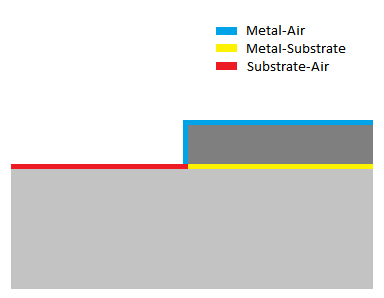
\includegraphics[scale=.8]{Figures/model}
\caption{Simplification of the system including three lossy layers. The substrate and metal are depicted in light and dark grey respectively}
\label{fig:model}
\end{figure}


\section{Ground}
To further reduce the number of mesh elements, the ground pad is replaced by a thin sheet of PEC. Considering the field in the ground region is small compared to the field at the edges of the pads its contribution to the participation ratio is also small. Investing more computation time on the ground region by increasing the density of mesh elements there would therefore also have limited impact on the participation ratio.
\section{title}
\chapter{Results and Discussion}
The starting point of this project was the familiar interdigitated qubit (see figure \ref{fig:Yale_parameters2}). This chapter will start with a discussion of the results gathered on this design.
%\cite{Houck2007}
%%The main focus during this project rested on two distinct qubit designs, namely the interdigitated and the parallel pad qubits. The two designs can be compared in figure \ref{fig:}.


First, the influence of different parameters on the capacitance of structures was determined. This knowledge enables designing structures with a specific capacitance necessary for a qubit with a certain frequency (see equation \eqref{eq:}). The target capacitance is 60 \(f\)F. With an inductor having an inductance of 10 \(n\)H this result in a resonance frequency of around 6.5 \(G\)Hz.


Secondly, the participation ratio of the lossy layers is determined. This will give insight into what design decisions can be made to reduce these participation ratios.\\
Taking these insights into account, a second qubit design was investigated in similar fashion. 

\vfill

\begin{figure}[h]
	\centering
	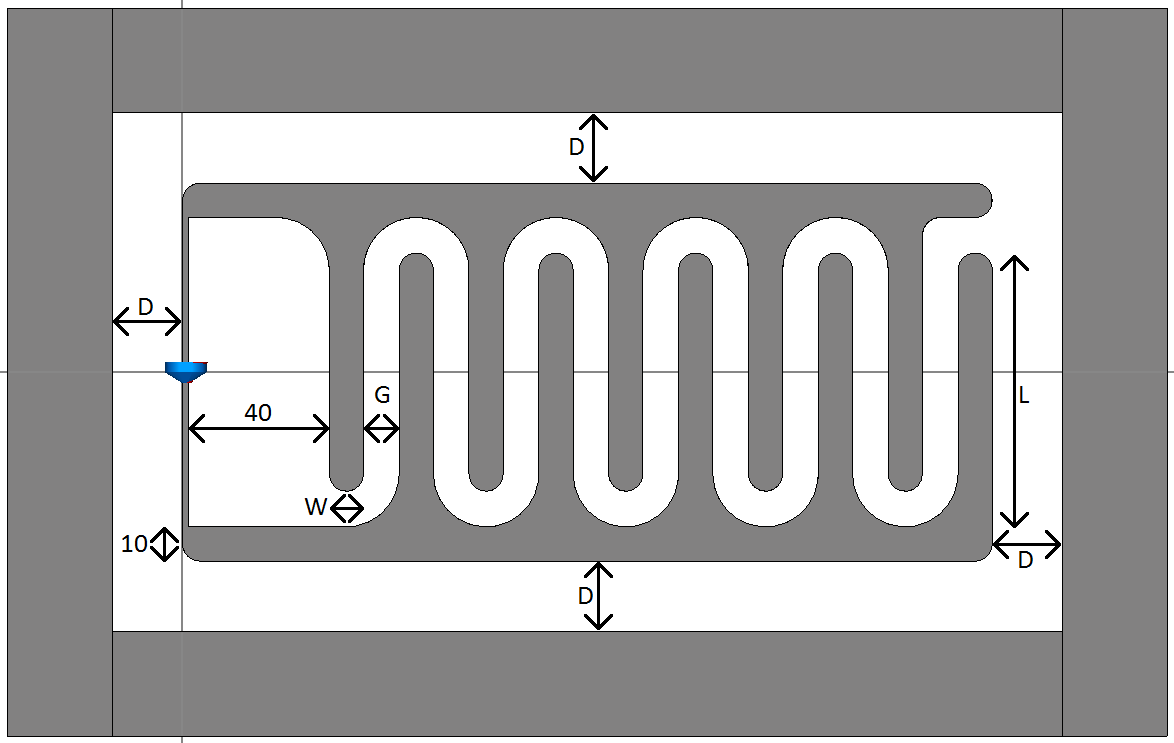
\includegraphics[scale = .4]{Figures/Yale_parameters2_cropped}
	\caption{The interdigitated qubit design including parameters and dimensions valid for all iterations of the design. Dimensions are in micrometers.}
	\label{fig:Yale_parameters2}
\end{figure}

\clearpage
\section{Interdigitated qubit}
As the name suggests the interdigitated qubit consists of two pads having a certain amount of fingers. The pads are positioned such that the fingers are at an equal distance from each other. The distance between the inductor and the first finger was set to 40 \(\mu\)m for all interdigitated qubit designs. An overview of the design with its parameters is depicted in figure \ref{fig:Yale_parameters2}




\subsection{The capacitance}
To better determine the influence of the pad design on the capacitance of the system, the influence of the ground plane is determined as a function of separation distance. Figure \ref{fig:capacitance_vs_slotsize} indicates that the influence of the ground plane on the capacitance of the system decreases rapidly with increasing separation distance. The influence of the ground plane becomes insignificant only at a separation distance of around 100 \(\mu\)m. So, in order to determine the influence of changes in pad design on the capacitance (and participation ratio) of the system, the separation distance of the ground plane should be carefully kept equal among pad designs. \todo{Or I should have eliminated the ground plane altogether when determining the influence of certain parameters.} 

\begin{figure}
	\centering
	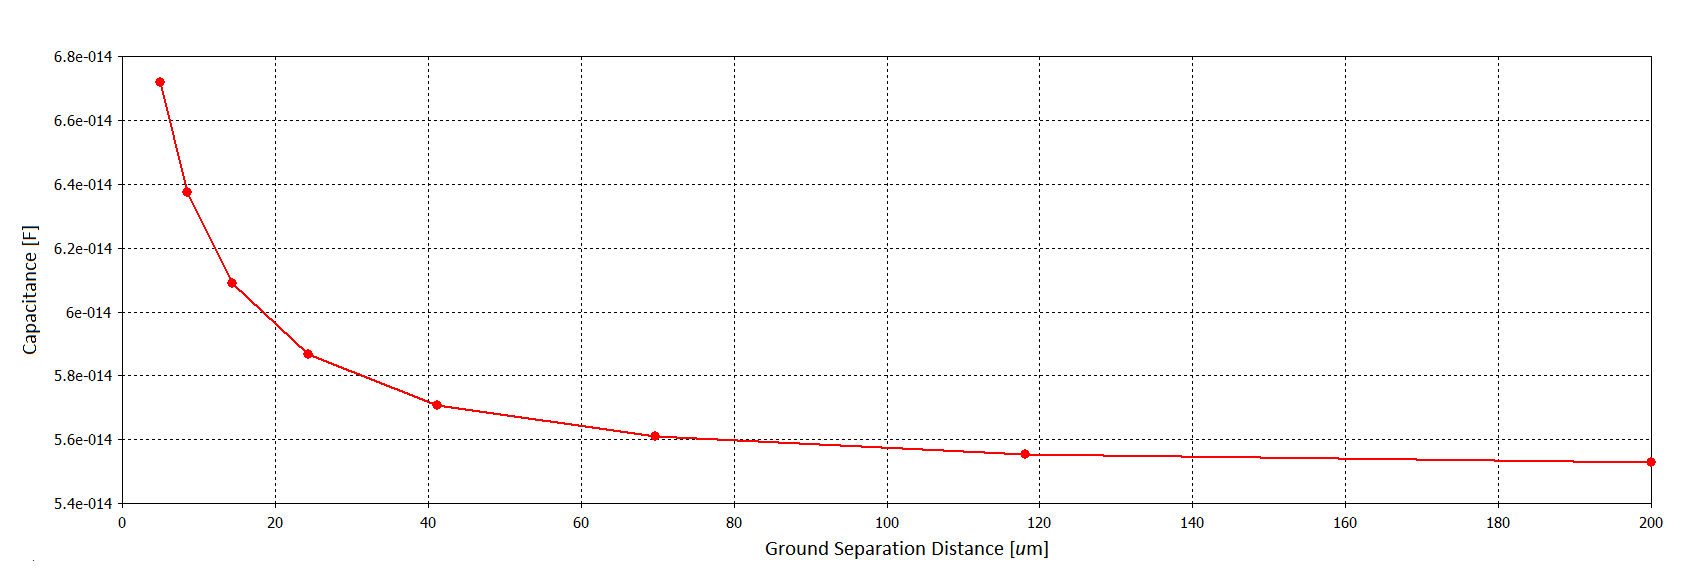
\includegraphics[width = \textwidth]{Figures/capacitance_vs_slotsize_edit}
	\caption{Capacitance of the system as a function of ground plane separation}
	\label{fig:capacitance_vs_slotsize}
\end{figure}

For the interdigitated pad design specifically, the first parameter under investigation is the amount of 'fingers' in the  qubit. The capacitances of qubits with 4 to 9 fingers were determined. The finger length, width and separation were not changed.
As can be seen in figure \ref{fig:CapVSFingers}, the relationship appears to be linear. This can be explained by viewing the addition of a finger as the addition of an extra capacitor in parallel.\\

\begin{figure}
	\centering
	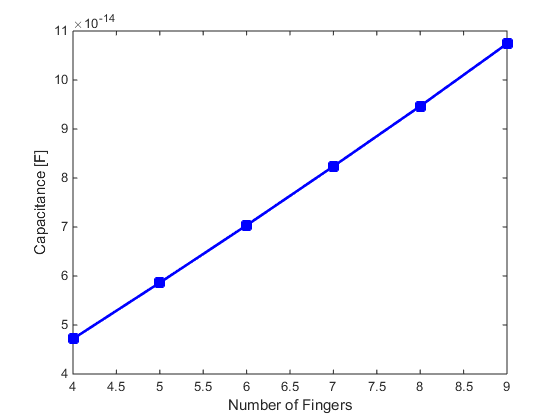
\includegraphics[scale = 0.7]{Figures/Capacitance_Plots/CapVSFingers.png}
	\caption{Capacitance as a function of the amount of fingers in the interdigitated qubit design. Finger width and length are equal in all qubits.}
	\label{fig:CapVSFingers}
\end{figure}

Next the influence of the finger width is determined. The finger separation is kept equal to the finger width. For a design with five fingers the results are depicted in figure \ref{fig:CapVSWidthL10}. \\

\begin{figure}
	\centering
	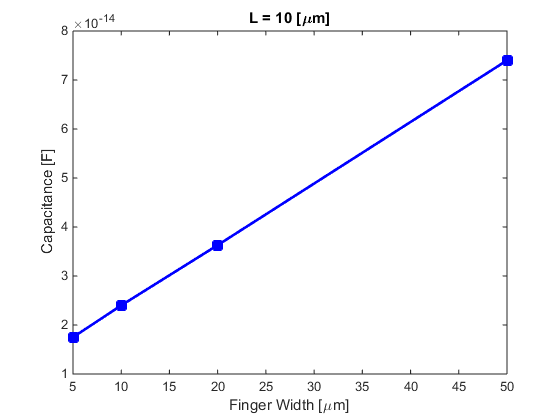
\includegraphics[scale = 0.7]{Figures/Capacitance_Plots/CapVSWidthL10.png}
	\caption{Capacitance as a function of finger width in the interdigitated qubit design. All qubit have five fingers and equal finger length.}
	\label{fig:CapVSWidthL10}
\end{figure}

Having determined the dependencies, qubits can be designed to have specific capacitances. Keeping all other parameters equal, the capacitance of earlier systems was tuned by adjusting the length of the fingers. For qubits with 5 fingers and a finger width of 5 to 50 \(\mu\)m the finger length was adjusted between 10 and 100 \(\mu\)m. \\
The results are combined in figure \ref{fig:Capacitances_g5_50}. From the figure it is possible to determine the finger length needed to achieve the target capacitance of 60 \(f\)F. For qubits with a finger width of  5 \(\mu\)m, 10 \(\mu\)m, and 20 \(\mu\)m, their length must be 87 \(\mu\)m, 76 \(\mu\)m, and 56 \(\mu\)m  respectively.   

\begin{figure}
	\centering
	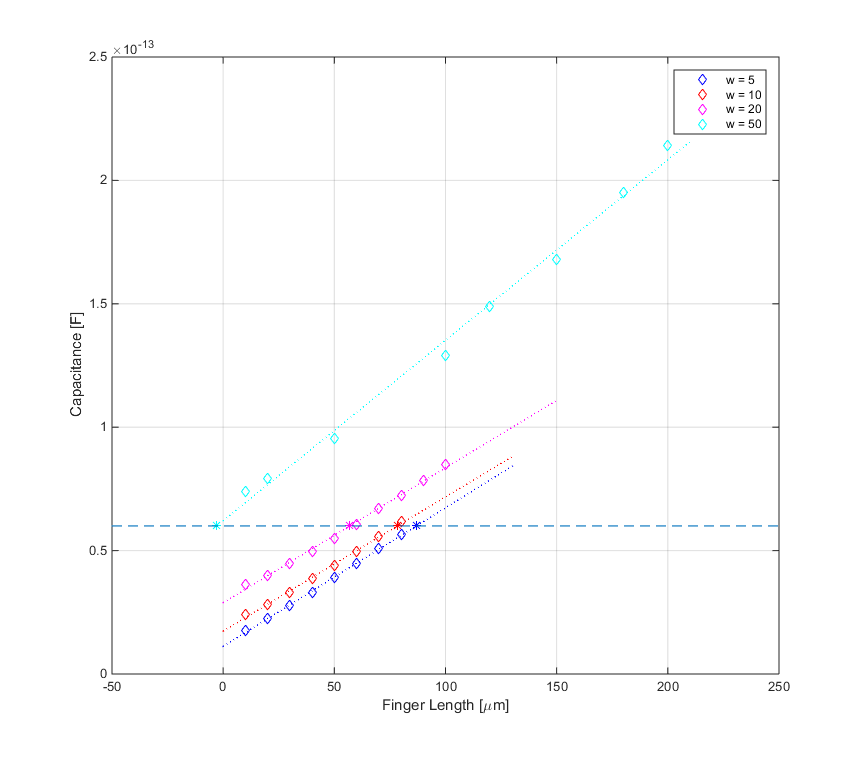
\includegraphics[width = \textwidth]{Figures/Capacitances_g5_50}
	\caption{A plot of the capacitance as a function of finger length for several finger widths. dotted lines represent linear fits of the data. The horizontal dashed line is a guideline for the eye showing the necessary finger length to make a 60\(f\)F capacitor; 87 \(\mu\)m, 76 \(\mu\)m, and 56 \(\mu\)m for qubits with a finger width of  5 \(\mu\)m, 10 \(\mu\)m, and 20 \(\mu\)m respectively.}
	\label{fig:Capacitances_g5_50}
\end{figure} 

\clearpage

 \begin{figure}
 	\centering
 	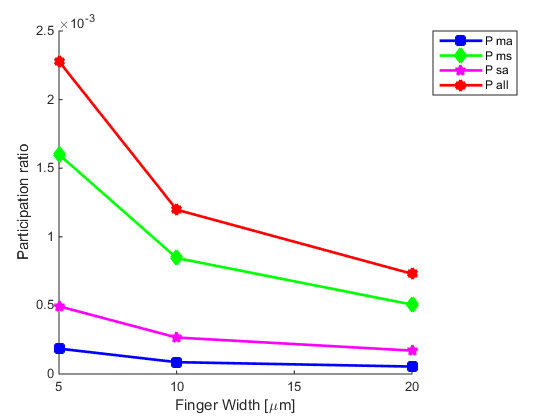
\includegraphics[scale = 0.7]{Figures/Ratio_plots/FingerWidth_legend}
 	\caption{A plot of the different ratios for qubits with five fingers.  The length of the fingers has been adjusted for each qubit to reach a capacitance of 60 \(f\)F. For qubits with a finger width of  5 \(\mu\)m, 10 \(\mu\)m, and 20 \(\mu\)m, their lengths are 87 \(\mu\)m, 76 \(\mu\)m, and 56 \(\mu\)m  respectively.}
 	\label{fig:FingerWidth_legend}
 \end{figure}

\subsection{The participation ratios}
Using the previous results several interdigitated qubits were designed to have a capacitance of 60 \(f\)F. An overview of the relevant parameters can be seen in table \ref{table:60fF_fingerlength}. The resulting participation ratios of the different lossy layers can be seen in the same table and are plotted in figure \ref{fig:FingerWidth_legend} for those qubits with 5 fingers. As the finger width is increased and the finger length decreased, all participation ratios decrease.

\begin{table}
	\begin{center}
		\begin{tabular}{ | l || c | c || c | c | c | c |}
			\hline
			Fingers  & Finger Width [\(\mu\)m] & Finger Length [\(\mu\)m]  & P ma &  Pms & P sa & P all \\ \hline
			5 & 5 & 87 & 1.85e-04 & 1.60e-03 & 4.94e-04 & 2.28e-03 \\  
			5 & 10 & 76 & 8.62e-05 & 8.45e-04 & 2.66e-04 & 1.20e-03 \\
			5 & 20 & 56 & 5.43e-05 & 5.06e-04 & 1.70e-04 & 7.31e-04  \\
			10 & 5 & 36 & 1.36e-04 & 1.30e-03 & 4.12e-04 & 1.85e-03 \\
			10 & 10 & 26 & 7.56e-05 & 7.33e-04 & 2.46e-04 & 1.06e-03 \\
			\hline
		\end{tabular}
	\end{center}
	\caption{The relevant parameters for interdigitated qubit and the resulting participation ratios. For all designs the finger length has been tuned to result in a qubit with a capacitance of 60 \(f\)F. }
	\label{table:60fF_fingerlength}
\end{table}



By default the corners of the fingers were rounded (as in figure \ref{fig:Yale_parameters2}). As this was not standard practice the influence of doing so was determined retroactively. To do so the corner radius of the fingers (with a width of 20 \(\mu\)m) was changed between 1 and 10 \(\mu\)m (10 \(\mu\)m making semi-circles at the finger tips). The resulting participation ratios can be seen in table \ref{table:ratio_cornerradius} and figure \ref{fig:CornerRadius}. All participation ratios tend to decrease as the corner radius is increased. 

 \begin{figure}
 	\centering
 	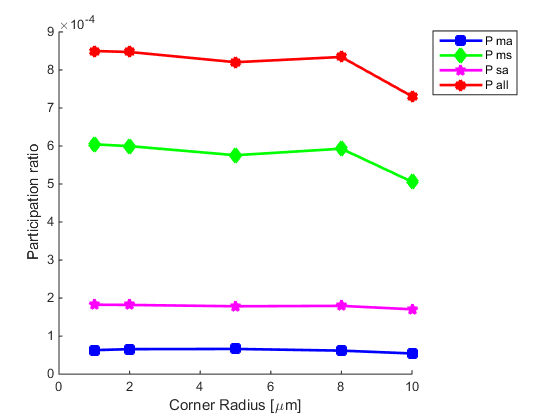
\includegraphics[scale = 0.7]{Figures/Ratio_plots/CornerRadius_legend}
 	\caption{A plot of the different participation for several corner radii. However slowly, all ratios tend to decrease with increasing radius.}
 	\label{fig:CornerRadius}
 \end{figure}

\begin{table}
	\begin{center}
		\begin{tabular}{ | l || c | c | c | c | c |}
			\hline
			Corner radius [\(\mu\)m] & P ma & P ms & P sa & P all \\ \hline
			1 & 6.30e-05 & 6.04e-04 & 1.83e-04 & 8.50e-04 \\
			2 & 6.57e-05 & 6.00e-04 & 1.82e-04 & 8.47e-04 \\
			5 & 6.62e-05 & 5.76e-04 & 1.78e-04 & 8.20e-04\\
			8 & 6.18e-05 & 5.93e-04 & 1.80e-04 & 8.34e-04\\
			10 & 5.43e-05 & 5.06e-04 & 1.70e-04 & 7.31e-04\\
			\hline
		\end{tabular}
	\end{center}
	\caption{The participation ratios for different corner radii.}
	\label{table:ratio_cornerradius}
\end{table}

The influence of the ground plane separation distance on the participation ratios was also determined. The distance was changed between 10 \(\mu\)m and 200 \(\mu\)m. The resulting participation ratios can be found in table \ref{table:ratio_groundseparation} and figure \ref{fig:SlotSize_legend}. Again, all participation ratios show a downward trend with increasing separation distance. The influence of increasing the the separation beyond 100 \(\mu\)m is very small.

 \begin{figure}
 	\centering
 	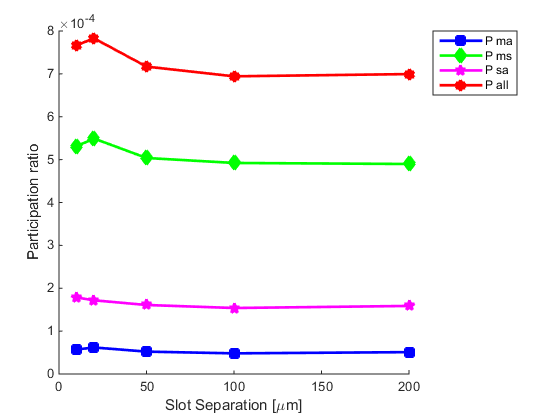
\includegraphics[scale = 0.7]{Figures/Ratio_plots/SlotSize_legend}
 	\caption{A plot of the different participation ratios for several separation distances to the ground plane. However slowly, all ratios tend to decrease with increasing separation.}
 	\label{fig:SlotSize_legend}
 \end{figure}

\begin{table}
	\begin{center}
		\begin{tabular}{ | l || c | c | c | c | c |}
			\hline
			Ground Separation [\(\mu\)m] & P ma & P ms & P sa & P all \\ \hline
			10 & 5.71e-05 & 5.31e-04 & 1.78e-04 & 7.67e-04 \\
			20 & 5.43e-05 & 5.06e-04 & 1.70e-04 & 7.31e-04 \\
			50 & 5.22e-05 & 5.04e-04 & 1.61e-04 & 7.17e-04 \\
			100 & 4.82e-05 & 4.92e-04 & 1.54e-04 & 6.94e-04 \\
			200 & 5.10e-05 & 4.90e-04 & 1.59e-04 & 7.00e-04\\
			\hline
		\end{tabular}
	\end{center}
	\caption{The participation ratios for different ground separation distances.}
	\label{table:ratio_groundseparation}
\end{table}

Looking at these results for the interdigitated qubit design it can be seen that the most significant change in participation ratios was achieved by making the fingers shorter and separating them further. Extrapolating these changes would indicate that a qubit consisting of two parallel rectangular pads would have even smaller participation ratios.

% \textit{Alternatively:}Extrapolating these changes would indicate that making the fingers ever shorter but wider would result in a qubit with even smaller participation ratios. The resulting qubit consists of two rectangular pads separated by the junction. 

\clearpage
\section{Parallel pad qubit}
The resulting qubit design can be seen in figure \ref{fig:IBM_parameters23}. It consists of two large parallel pads which are connected two smaller pads with the inductor in-between. The ground plane consist of a square slot at a relatively large distance from the qubit. Due to its simplicity, there are fewer ways of changing the qubit. The parameters under consideration are the pad separation, the pad width, and the radius of the corners. Again, first, the influence different parameters have on the capacitance of the system was determined. Afterwards the participation ratios of different configurations were calculated.

\begin{figure}[h]
	\centering
	\begin{tabular}{c}
		\subfloat[Overview of the parallel pad qubit]{{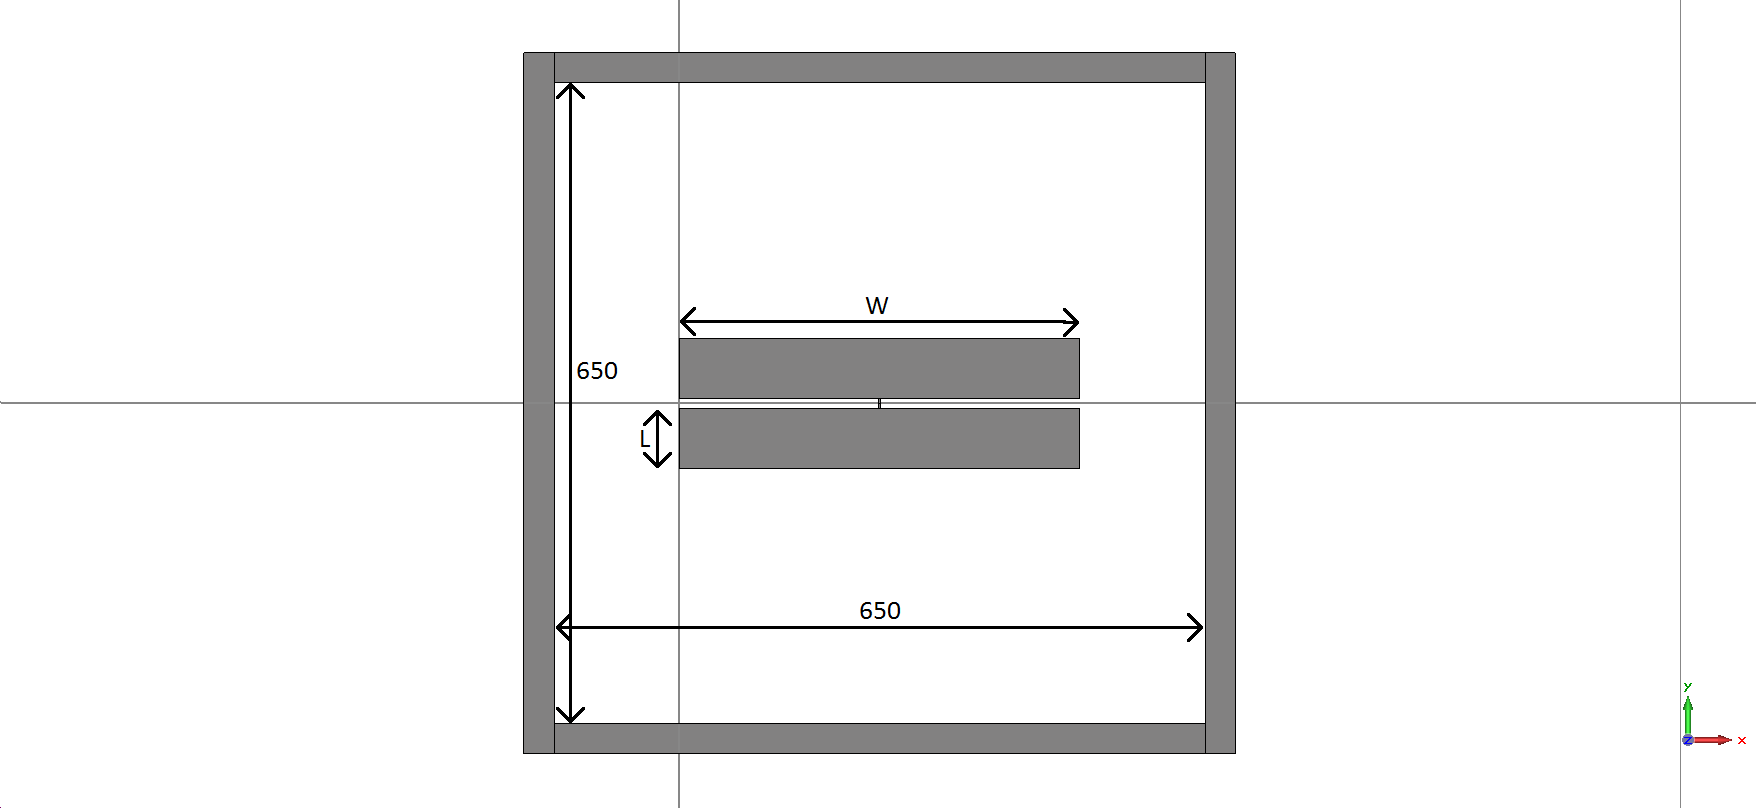
\includegraphics[width = \textwidth]{Figures/IBM_parameters3} }} \\
		
		\subfloat[Zoomed in view of the center of the qubit.]{{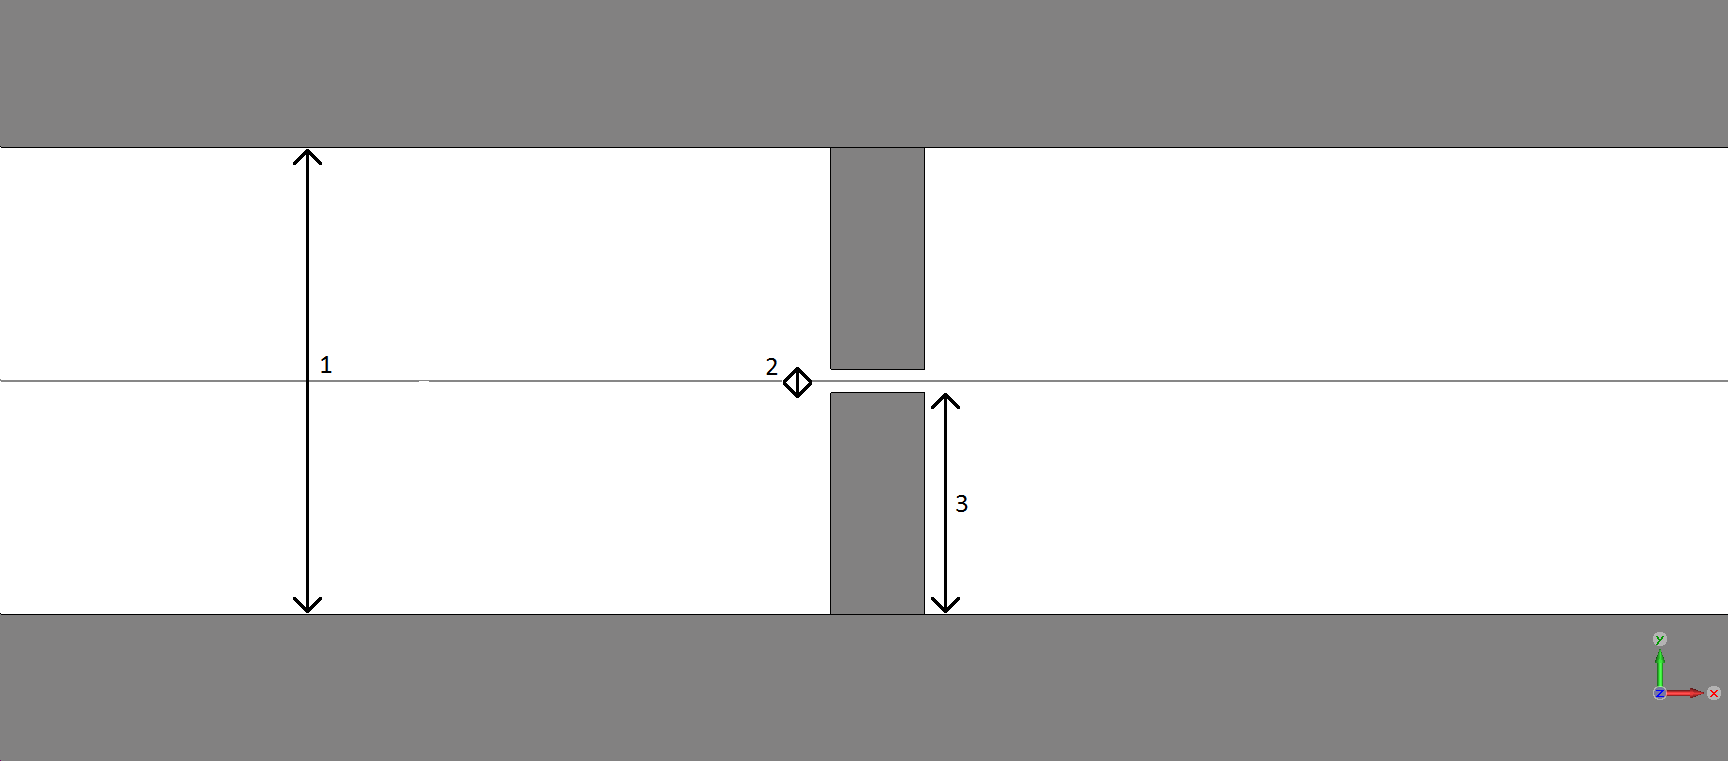
\includegraphics[width = \textwidth]{Figures/IBM_parameters2} }}
	\end{tabular}
	\caption{The parallel pad qubit design including parameters and dimensions valid for all iterations of the design. (a) W is the width of the pads, L is the length of the pad, the size of the grounded slot here is 650 \(\mu\)m. (b) 1 is the pad separation distance. 2 is the junction separation distance which is 0.5 \(\mu\)m for all qubits. 3 is the length of the junction lead which depends only on the separation distance of the qubit.}
	\label{fig:IBM_parameters23}
\end{figure}



\subsection{The capacitance}
Similar to adding extra fingers to the interdigitated qubit, widening the pad width is expected to linearly increase the capacitance of the system. The pad width was changed between 300 and 500 \(\mu\)m. The data shown in figure \ref{fig:IBMCapVSWidth} indeed shows a linear proportionality.

\begin{figure}
	\centering
	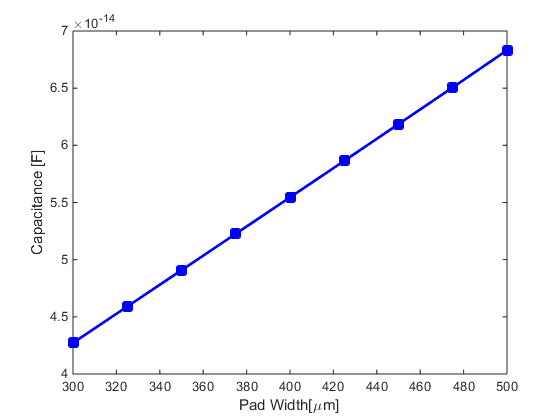
\includegraphics[scale = 0.7]{Figures/Capacitance_plots/IBMCapVSWidth}
	\caption{The capacitance of parallel pad qubits with different pad widths.}
	\label{fig:IBMCapVSWidth}
\end{figure}

The capacitance of a standard parallel plate capacitor is inversely proportional to the plate separation. Similar proportionality is expected for the parallel pad qubit system. The pad separation was set between 5 and 60 \(\mu\)m. The resulting capacitances can be seen in figure \ref{fig:IBMCapVSPadSep}.

Finally the radius of pads' corners are changed. They were set between 5 and 30 \(\mu\)m. The resulting capacitances are shown in figure \ref{fig:IBMCapVSCornerRadius}.

\begin{figure}[h]
	\centering
	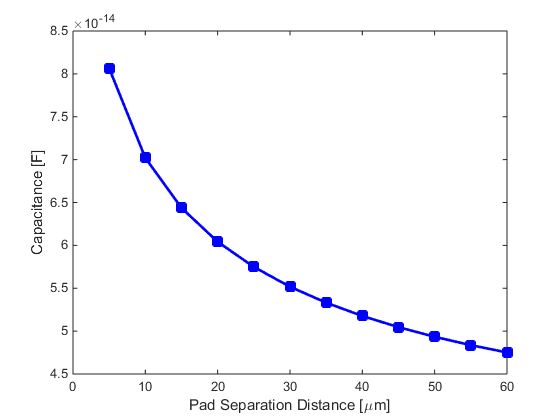
\includegraphics[scale = 0.7]{Figures/Capacitance_plots/IBMCapVSPadSep}
	\caption{The capacitance of parallel pad qubits with different pad separation distances.}
	\label{fig:IBMCapVSPadSep}
\end{figure}


\begin{figure}
	\centering
	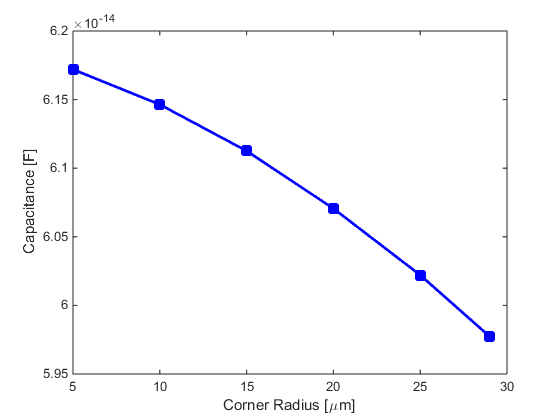
\includegraphics[scale = 0.7]{Figures/Capacitance_plots/IBMCapVSCornerRadius}
	\caption{The capacitance of parallel pad qubits with different corner radii.}
	\label{fig:IBMCapVSCornerRadius}
\end{figure}

\clearpage
\subsection{The participation ratios}
 %The influence of the pad separation and the pad width on the participation ratios of the layers were determined. 
 Comparing the two qubit designs; increasing the finger width (and separation) in the interdigitated qubit can be seen as increasing the pad separation and pad width in the parallel pad qubit. Therefore the participation ratios are expected to decrease when increasing pad width or separation. The influence of three parameters on the participation ratios were investigated separately: the pad separation, the pad width, and the corner radius. Contrary to what was done during the investigation of the interdigitated qubit, the resonance frequencies of all parallel pad qubits were kept equal by changing the value of the inductance (see formula \eqref{eq:}). 
 
 Starting with the pad width which was again changed between 300 and 500 \(\mu\)m. Table \ref{table:ratio_IBMPadWidth} and figure \ref{fig:IBMPadWidth_legend} show the resulting ratios, all of them decreasing with increasing width.
 
 \begin{table}
 	\begin{center}
 		\begin{tabular}{ | l || c | c | c | c | c |}
 			\hline
 			Pad Width [\(\mu\)m] & P ma & P ms & P sa & P all \\ \hline
 			300 & 4.71e-05 & 3.51e-04 & 1.08e-04 & 5.06e-04 \\
 			350 & 4.29e-05 & 3.44e-04 & 1.04e-04 & 4.91e-04 \\
 			400 & 4.27e-05 & 3.38e-04 & 1.02e-04 & 4.82e-04 \\
 			450 & 4.17e-05 & 3.32e-04 & 1.01e-04 & 4.74e-04 \\
 			500 & 4.04e-05 & 3.28e-04 & 9.92e-05 & 4.68e-04\\
 			\hline
 		\end{tabular}
 	\end{center}
 	\caption{The participation ratios of parallel pad qubits with different pad widths.}
 	\label{table:ratio_IBMPadWidth}
 \end{table}
 
 \begin{figure}
 	\centering
 	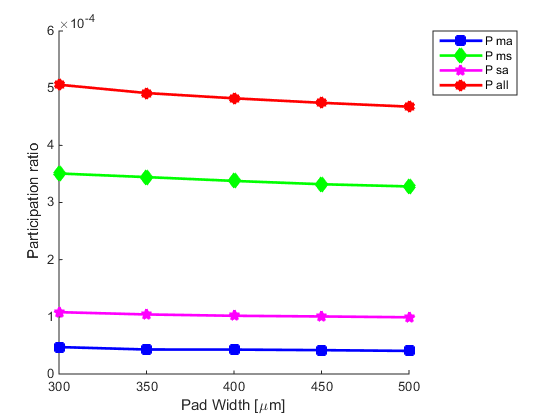
\includegraphics[scale = 0.7]{Figures/Ratio_plots/IBMPadWidth_legend}
 	\caption{The participation ratios of parallel pad qubits with different pad widths.}
 	\label{fig:IBMPadWidth_legend}
 \end{figure}
 
 Secondly, the separation between the two pads was changed between 5 and 60 \(\mu\)m. The results in table \ref{table:IBMPadSep} and figure \ref{fig:IBMPadSep_legend} again show decreasing ratios for all layers with increasing separation. 
 
 \begin{table}
 	\begin{center}
 		\begin{tabular}{ | l || c | c | c | c | c |}
 			\hline
 			Pad Separation [\(\mu\)m] & P ma & P ms & P sa & P all \\ \hline
 			5 & 6.42e-05 & 5.59e-04 & 1.82e-04 & 8.42e-04 \\
 			10 & 4.65e-05 & 4.26e-04 & 1.28e-04 & 6.00e-04 \\
 			20 & 4.02e-05 & 3.21e-04 & 9.67e-05 & 4.58e-04 \\
 			50 & 3.35e-05 & 2.55e-04 & 7.70e-05 & 3.65e-04 \\
 			\hline
 		\end{tabular}
 	\end{center}
 	\caption{The participation ratios of parallel pad qubits with different pad separation distances.}
 	\label{table:IBMPadSep}
 \end{table}
 
 \begin{figure}
 	\centering
 	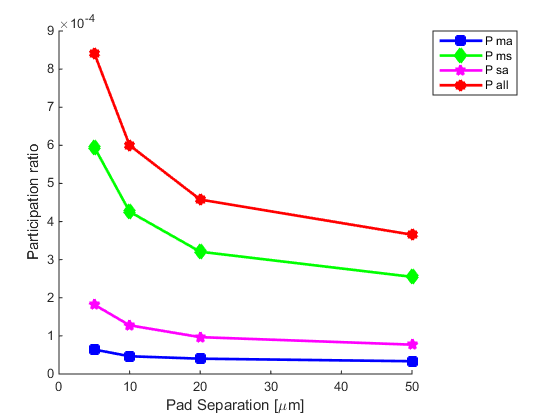
\includegraphics[scale = 0.7]{Figures/Ratio_plots/IBMPadSep_legend}
 	\caption{The participation ratios of parallel pad qubits with different pad separation distances.}
 	\label{fig:IBMPadSep_legend}
 \end{figure}
 
 Finally, the radius of the corners was changed between 5 and 30 \(\mu\)m, where a radius of 30 \(\mu\)m results in an semi-circle on the sides. Although the resulting ratios in table \ref{table:IBMCornerRadius} and figure \ref{fig:IBMCornerRadius_legend} show a decreasing trend, the change is much less significant compared to that of the interdigitated qubit.
 
 \begin{table}
 	\begin{center}
 		\begin{tabular}{ | l || c | c | c | c | c |}
 			\hline
 			Corner Radius [\(\mu\)m] & P ma & P ms & P sa & P all \\ \hline
 			5 & 3.74e-05 & 3.03e-04 & 9.53e-05 & 4.35e-04 \\
 			10 & 3.56e-05 & 3.01e-04 & 9.47e-05 & 4.31e-04 \\
 			15 & 3.67e-05 & 2.98e-04 & 9.60e-05 & 4.31e-04 \\
 			20 & 3.37e-05 & 3.00e-04 & 9.51e-05 & 4.29e-04 \\
 			25 & 3.47e-05 & 2.97e-04 & 9.41e-05 & 4.26e-04 \\
 			29 & 3.49e-05 & 2.99e-04 & 9.47e-05 & 4.28e-04 \\
 			\hline
 		\end{tabular}
 	\end{center}
 	\caption{The participation ratios of parallel pad qubits with different corner radii.}
 	\label{table:IBMCornerRadius}
 \end{table}
 
 \begin{figure}
 	\centering
 	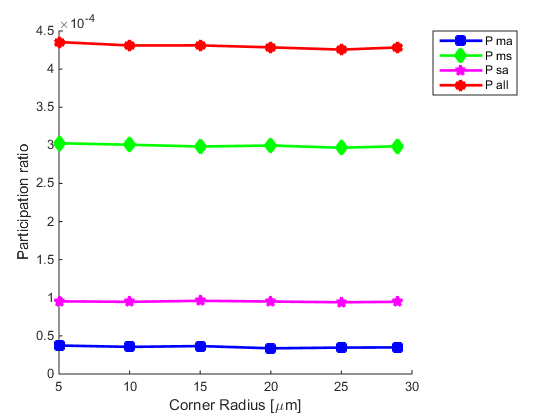
\includegraphics[scale = 0.7]{Figures/Ratio_plots/IBMCornerRadius_legend}
 	\caption{The participation ratios of parallel pad qubits with different corner radii.}
 	\label{fig:IBMCornerRadius_legend}
 \end{figure}
 
\clearpage
\section{Further Discussion}
Finally, to explain some of the results, the simulated electric fields can be looked at. Figure \ref{fig:CornerFields} shows the absolute value of the electric field around the corners of the interdigitated (a and b) and parallel pad qubits (c and d). The electric field is less concentrated when the corners are rounded. It appears these highly concentrated electric fields at the corners are a cause for higher participation ratios. The reduction of the participation ratios is most apparent for the interdigitated qubit which simply has more corners.

 \begin{figure}
 	\begin{tabular}{c c}
 		\subfloat[Interdigitaded, finger slightly rounded]{{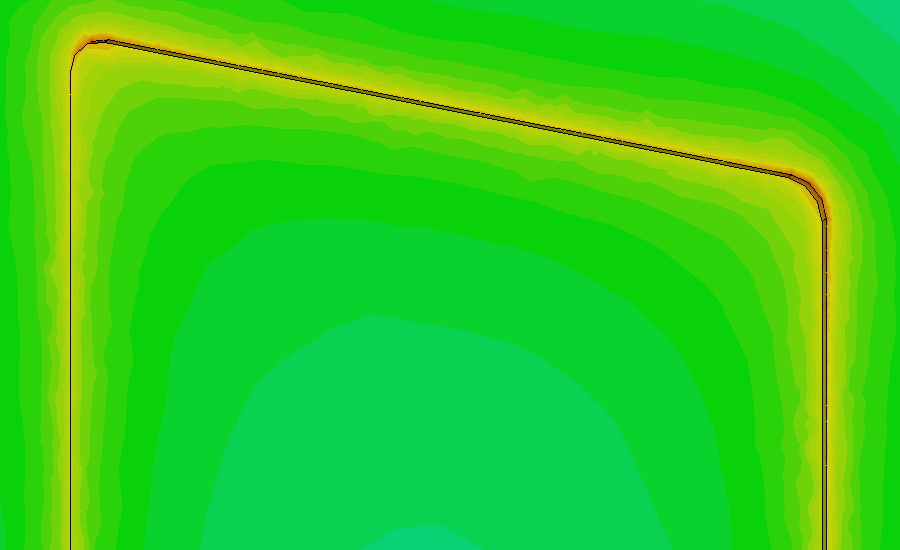
\includegraphics[width = \textwidth/2]{Figures/Fields/slightly_rounded_zoomed_cropped} }} & \subfloat[Interdigitaded, finger fully rounded]{{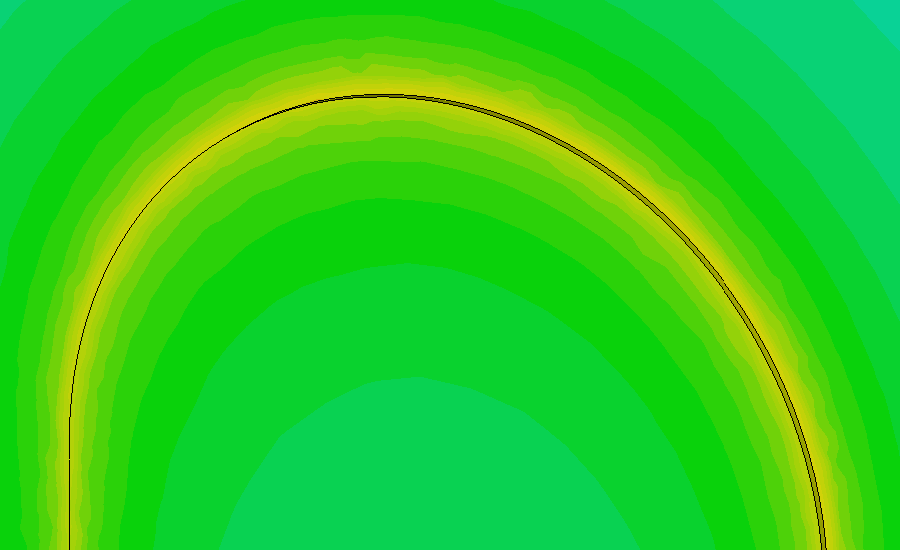
\includegraphics[width = \textwidth/2]{Figures/Fields/fully_rounded_zoomed_cropped} }} \\
 		\subfloat[Parallel pad, sharp corner]{{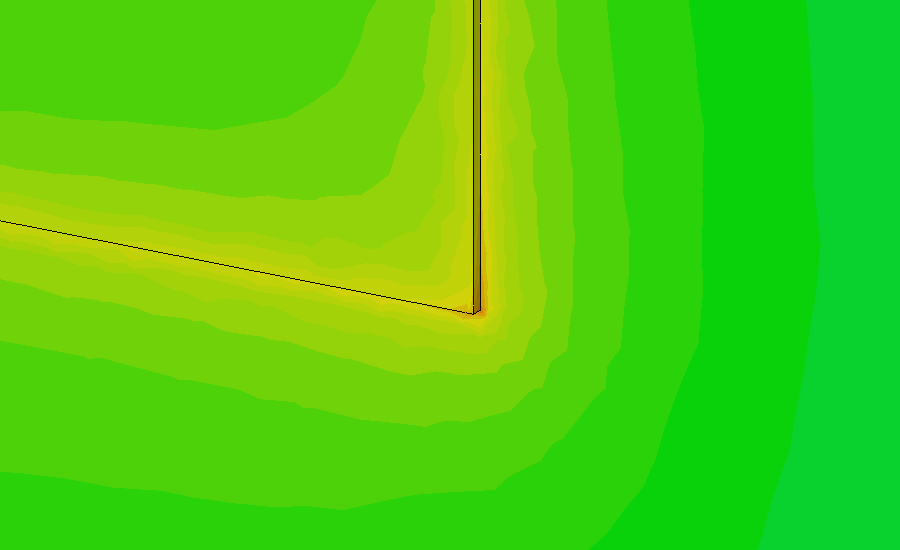
\includegraphics[width = \textwidth/2]{Figures/Fields/IBM_sharp_corner_cropped} }} & \subfloat[Parallel pad, rounded corner]{{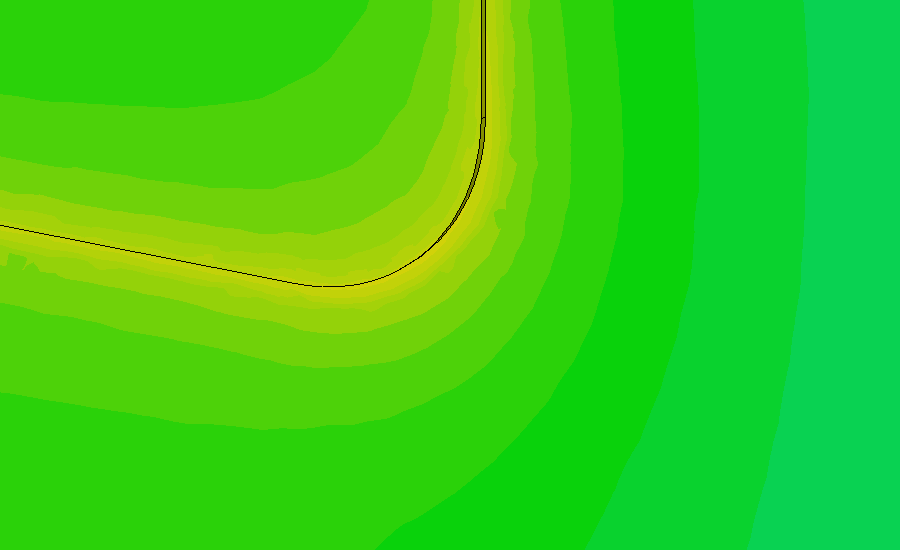
\includegraphics[width = \textwidth/2]{Figures/Fields/IBM_rounded_corner_r5_cropped} }}
	 \end{tabular}	
 	\centering	
 	\caption{The absolute value of the electric field in the area around corners. The rounding of the corners results in less concentrated electric fields.}
 	\label{fig:CornerFields}
 \end{figure}

 
Figure \ref{fig:} shows a the electric field on a cross-section of the parallel pad qubit with different pad separation distances, XXX \(\mu\)m away from the junction.


%\section{Conclusion} %Grafieken niet in de conclusie! hier geen nieuwe informatie geven!
%To explain these results the actual electric field can be looked at. Figure \ref{fig:} shows a comparison of the electric field intensity belonging to parallel pad qubits with a width of 300 and 500 \(\mu\)m. \todo{Explain differences in field intensity}.
% 
%Next, figure \ref{fig:} shows a comparison of the electric field intensity belonging to parallel pad qubits with a separation distance of 5 and 60 \(\mu\)m, a cross-section is also included. \todo{Explain differences in field intensity}.
% 
%Finally, figure \ref{fig:} shows a comparison of the electric field intensity belonging to both interdigitated and parallel pad qubit having partial of fully rounded corners. The difference is especially noticeable for the interdigitated qubits. \todo{Explain differences in field intensity}.
  




    

%% Use letters for the chapter numbers of the appendices.
\appendix

%\input{appendix-a}

\bibliography{report}
\begin{appendices}
	\chapter{CST procedure}
This chapter will detail the steps that should be taken to easily set up a qubit simulation in CST. First a project template needs to be created.
\section{Creating a new project}
 When a new project is started, CST asks which module is going to be used. Most settings can be changed at a later time.
 \begin{itemize}
 	\item After clicking '\textit{Create project}' choose '\textit{MW \& RF \& Optical}'.
 	\item Choose '\textit{Antennas}' and click '\textit{Next >}'.
 	\item Choose '\textit{Waveguide (Horn, Cone, etc.)}'.
 	\item Choose '\textit{Frequency Domain}'.
 	\item Select the units to be used, the default settings are sufficient.
 	\item Choose a frequency domain. This can be left blank and changed at a later time.
 	\item Click '\textit{Next}' to see an overview of the created template.
 	\item Click '\textit{Finish}'. 
 \end{itemize}
Qubit designs can now be imported or created in CST.\\

The estimation of the capacitance of the qubit and the electric fields in the structure will be treated separately as the second process is more complex. Both simulations make use of the Frequency Domain Solver. Settings applicable to both processes are the frequency range and the boundaries. 
\begin{itemize}
	\item Under '\textit{Simulation}' click '\textit{Frequency}' and set the desired values.
	\item Again under '\textit{Simulation}' click '\textit{Boundaries}' and set the fields as in figure \ref{fig:Boundaries}
	\item Click '\textit{Open Boundary...}' and under '\textit{Automatic minimum distance to structure}' select '\textit{Fraction of wavelength}' and set to 8. Click '\textit{OK}'.
\end{itemize}

\begin{figure}[h]
	\begin{center}
		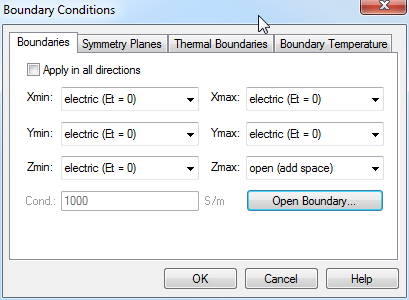
\includegraphics[scale = .7]{Figures/Boundaries}
		\caption{Settings for the boundary conditions of the simulations. All except '\textit{Zmax}' are set to '\textit{electric (Et = 0)}'. '\textit{Zmax}' is set to '\textit{open(add space)}'.}
		\label{fig:Boundaries}
	\end{center}
\end{figure}

\section{The capacitance}
As shown in equation \eqref{eq:totalenergy} the capacitance of the structure must be known to calculate the total energy in the qubit. The value of the capacitance converges very quickly as the mesh is refined. This simulation should always include a Discrete Port connected to the capacitor pads.
\begin{equation} \label{eq:totalenergy}
W=\frac{1}{2}CV^{2}
\end{equation}
Where \(C\) is the total capacitance of the system and \(V\) the voltage over the systems.

% 
\subsection{Modeling}
The qubit design can be imported to CST or created in CST itself. Figure \ref{fig:capacitance_basic_setup} shows a qubit designed in CST. It includes two perfectly electrical conducting (PEC) pads connected by a discrete port. The pads must be modelled using their actual thickness in order to include the lossy layers on their sides. A discrete port can be added as follows:
\begin{itemize}
	\item Under '\textit{Simulation}' click '\textit{Discrete Port}'.
	\item Now select the location in the model or input the coordinates numerically. Ensure that the discrete port connects the two PEC pads. 
	\item Leave all other settings as default.  
\end{itemize}
The pads are surrounded by a PEC ground sheet.
\begin{figure}
	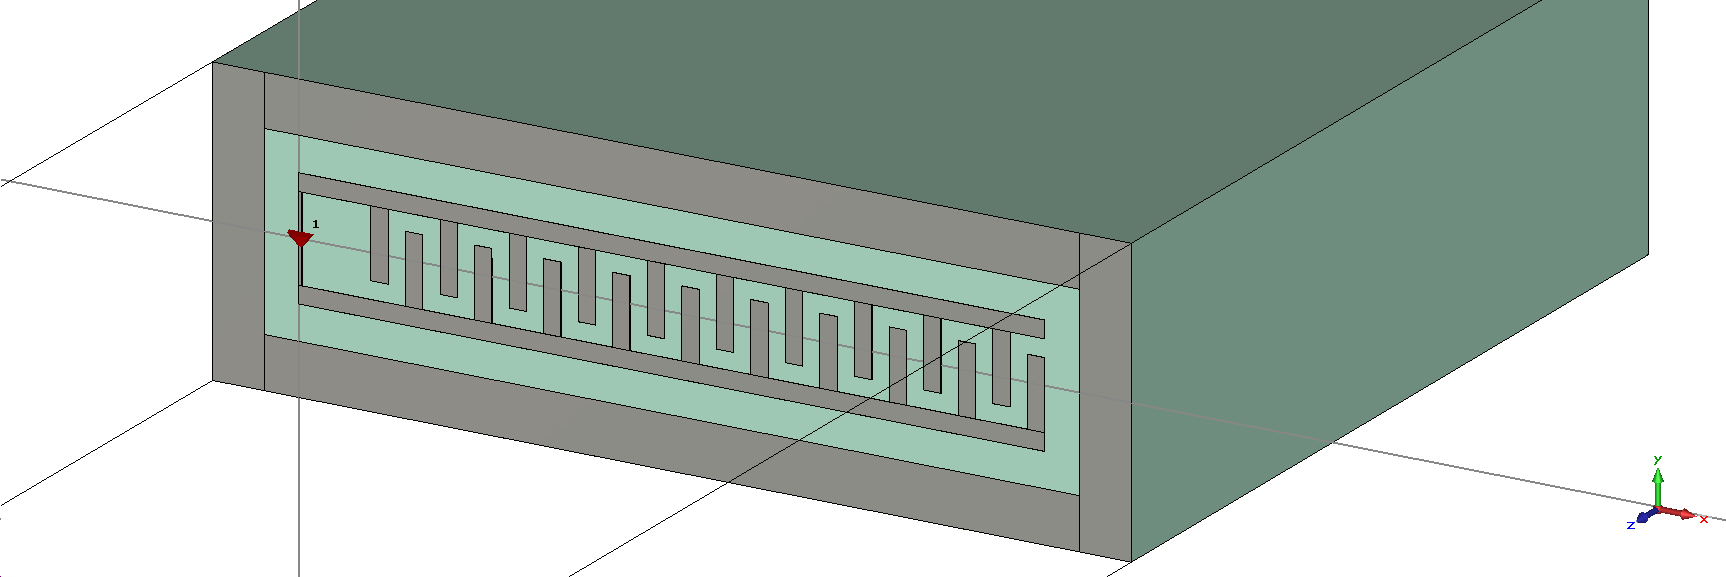
\includegraphics[width=\textwidth]{Figures/capacitance_basic_setup}
	\caption{An example of a qubit design with the substrate in green, the metal parts in grey and the port indicated by the red cone. No lumped element representing the Josephson junction is present in the model.}
	\label{fig:capacitance_basic_setup}
\end{figure}
For the determination of the capacitance, the inductor representing the Josephson junction should be omitted from the simulation.
\subsection{Meshing}
The default settings for the tetrahedral meshing can be used during calculation of the capacitance. This will yield a very rough initial mesh with few mesh elements and will ensure short simulation times.
\subsection{Post processing}
In the post processing templates window, the capacitance of the simulated structure can be retrieved; 
\begin{itemize}
	\item Under '\textit{Post Processing}' select '\textit{Template Based Post Processing}'.
	\item In the pop-up window, in the first selection box choose '\textit{S-Parameters}'.
	\item In the second selection box choose '\textit{Z-parameter}'.
	\item In the pop-up window check the '\textit{C}' option and click '\textit{OK}'.
\end{itemize}
This will yield a 2D graph showing the capacitance of the structure as a function of frequency. \\
Now include a second template;
\begin{itemize}
	\item In the first selection box choose '\textit{General 1D}'.
	\item In the second selection box choose '\textit{0D or 1D Results from 1D Result (Rescale, Derivation, etc)}'.
	\item In the pop-up window select '\textit{y at given x}' and set '\textit{Evaluate at x =}' to the desired frequency. Click '\textit{OK}'.
\end{itemize}
After simulation, the result should be a single value of the capacitance at the required frequency.

\subsection{Simulation setup}
To ensure convergence of the capacitance, results from the post processing templates can be used as targets for the simulation;
\begin{itemize}
	\item Under '\textit{Simulation}' choose '\textit{Setup Solver}'.
	\item Under '\textit{Adaptive mesh refinement}' make sure the '\textit{Adaptive tertrahedral mesh refninement}' is checked and click '\textit{Properties}'.
	\item In the pop-up window under '\textit{Number of passes}' set the maximum to at least 8.
	\item Under '\textit{Check after broadband calculation:}' mark the '\textit{OD result Template...}' as active and select the 0D result of the capacitance from the post processing template above. 
	\item Set the required Treshold and Checks as desired and click '\textit{OK}'.
\end{itemize}
This will ensure the simulation keeps refining the mesh until your demands on accuracy are met or until maximum amount of mesh refinement passes is reached. After every mesh refinement pass the results are updated and can be checked. In the Navigation Tree click '\textit{Tables}' \(\rightarrow\) '\textit{0D Results}' \(\rightarrow\) '\textit{C1,1\_0D\_yAtX}'. The first result will be viewable once the first pass of the simulation is completed. When the simulation is finished the capacitance of the structure can extracted from the plot. An example is given in figure \ref{fig:capacitanceplot}.

\begin{figure}
	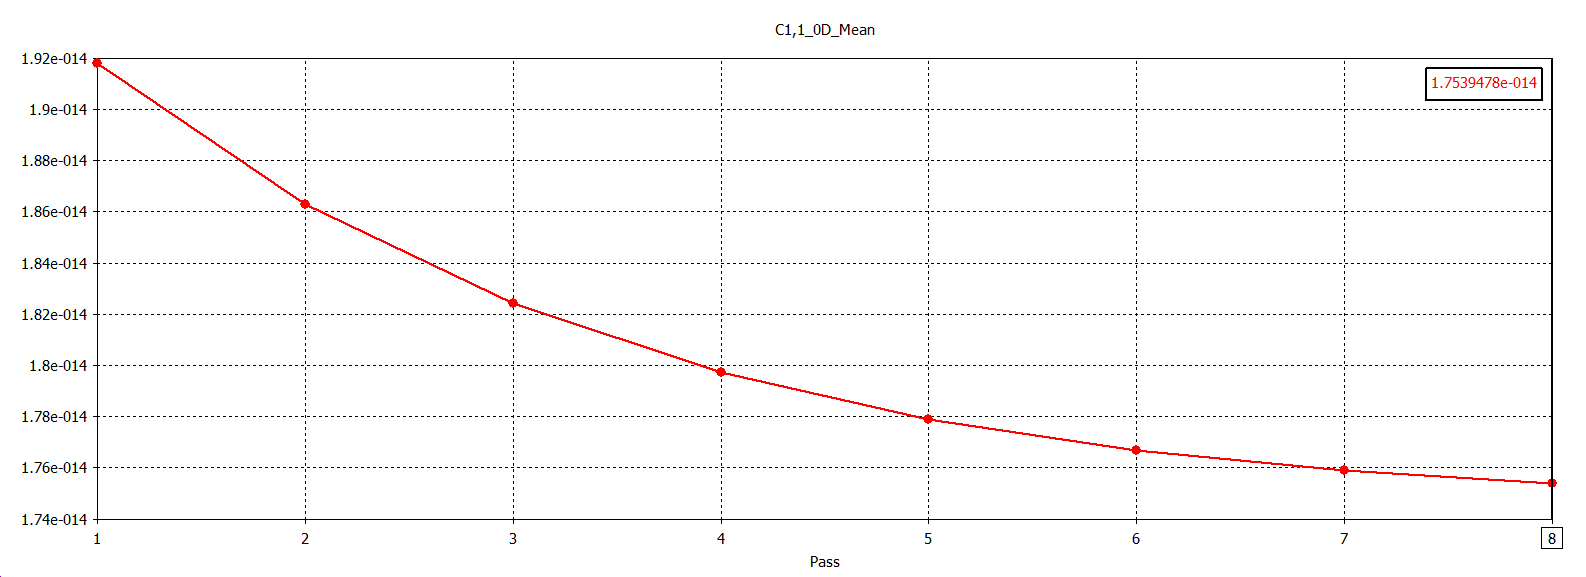
\includegraphics[width=\textwidth]{Figures/capacitanceplot}
	\caption{An example of the data retrieved on the capacitance of a qubit design. On the y-axis is the capacitance in Farad. On the x-axis is the number of mesh refinement passes. Highlighted is the value of the capacitance after 8 passes.}
	\label{fig:capacitanceplot}
\end{figure}

\section{The electric field}
Now that the capacitance of the structure is known the more extensive simulation of the electric field can be set up.
\subsection{Modeling}
Using equation \eqref{eq:impedance} the inductance needed to reach a certain resonance frequency can be calculated. 

\begin{equation}\label{eq:impedance}
L = \frac{1}{(2\pi)^{2}f_{0}^{2}C}
\end{equation}
Where \(f_{0}\) is the required qubit frequency and \(C\) its capacitance.\\
Now to include such an inductor;
\begin{itemize}
	\item In the simulation menu add a '\textit{Lumped element}'.
	\item Set the element '\textit{Type}' to be '\textit{RLC parallel}'
	\item Set the value of the inductance as calculated and leave the other values at zero.
	\item Make sure the '\textit{Monitor voltage and current}' is checked.
	\item Set the location as desired or use picked points.
\end{itemize}

Next, to ensure a fine initial mesh, the edges on the side of the pads are rounded. In order to make this possible each pad must be a single object. To achieve this the '\textit{Boolean}' operation can be used to combine multiple object into one;

\begin{itemize}
	\item In the Navigation Tree, under '\textit{Components}' select all objects pertaining to one pad.
	\item Under '\textit{Modeling}' click '\textit{Boolean}'.
\end{itemize}
Now that the pad consists of a single object, its side edges can be rounded.
\begin{itemize}
	\item Under '\textit{Modeling}' click '\textit{Picks}' and choose '\textit{Pick Edge Chain}' (or use Shift+E)
	\item Select all the edges laying in the \(xy\)-plane.
\end{itemize}
Figure \ref{fig:blending} show what the selection should look like. Once the right edges are selected they can be rounded;
\begin{itemize}
	\item Under '\textit{Modeling}' click '\textit{Blend}'.
	\item Set the '\textit{radius}' to be half the height of the pad. 
\end{itemize}
The result should be as in figure \ref{fig:blending}.


\begin{figure}[h]
	\centering
	\subfloat[A selection of two Edge Chains in red. One at the level of the substrate and another at the level of the top of the pad.]{{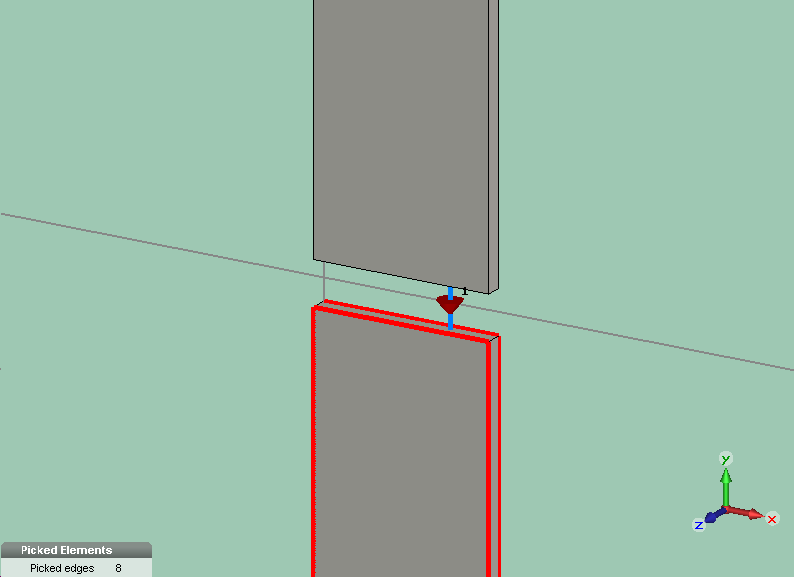
\includegraphics[width=5cm]{Figures/blending3} }}
	\qquad
	\subfloat[The resulting blended edges.]{{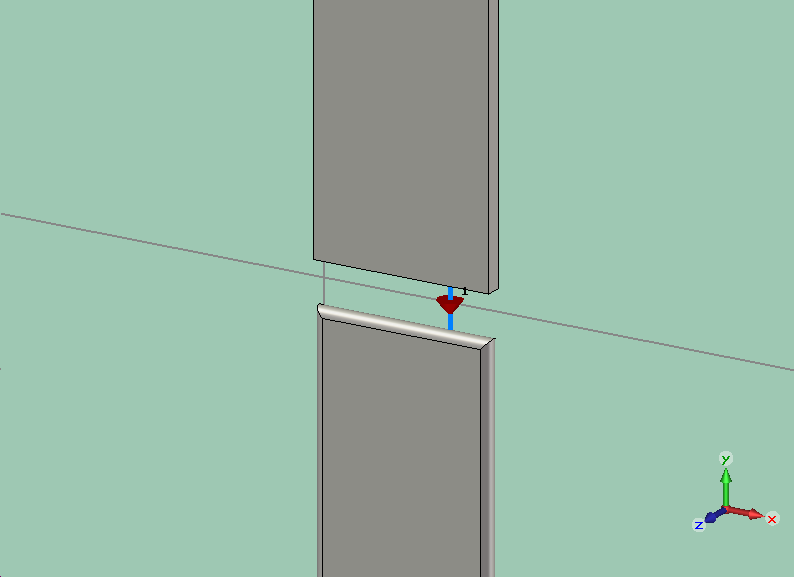
\includegraphics[width=5cm]{Figures/blending4} }}
	\caption{Before and after blending the edges}
	\label{fig:blending}
\end{figure}


\subsection{Meshing}
In order to obtain a fine initial mesh the \textit{Global mesh properties} can be changed;
\begin{itemize}
	\item Under '\textit{Simulation}' click '\textit{Global mesh properties}'.
	\item In the pop-up window click '\textit{Specials}'.
	\item Under the '\textit{Mesh Control}'-tab set '\textit{Smooth mesh with equilibrate ratio}' to around \(1.15\). Use this value to fine tune the number of mesh elements in the initial mesh.
	\item Set '\textit{Normal tolerance}' to \(1\) degree.
	\item \textbf{Uncheck} the '\textit{Anistropic curvature refinement}'. 
	\item Click '\textit{OK}' and '\textit{Update}' to see the resulting mesh. 
\end{itemize}

Again, use the '\textit{Smooth mesh with equilibrate ratio}' to tune the amount of mesh elements in the initial mesh.
See figure \ref{fig:MeshProperties} for the settings.
\begin{figure}[h]
	\begin{center}
		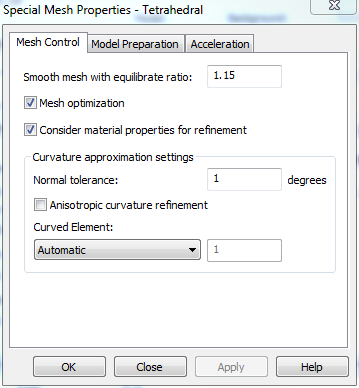
\includegraphics[scale = .6]{Figures/MeshProperties}
		\caption{The required settings for the Mesh Properties. The Anistropic curvature refinement must be unchecked!}
		\label{fig:MeshProperties}
	\end{center}
\end{figure}

\subsection{Simulation setup}
To be able to view and save field data, include a field monitor;
\begin{itemize}
	\item Under '\textit{Simulation}' click '\textit{Field Monitor}'.
	\item In the pop-up window select the E-Field monitor and choose a frequency.
	\item Click '\textit{OK}', the monitor should be visible in the Navigation Tree.
\end{itemize}
The simulation is now ready to run.

\subsection{Exporting data}
To calculate the participation ratio the simulated electric field is exported as an ASCII file. In order to separate data pertaining to different lossy layers the data for the field on the Pads, Substrate and Ground must be exported separately. 
\begin{itemize}
	\item In the Navigation Tree under '\textit{Components}' hide all objects until only the Pads are visible.
	\item Again in the Navigation Tree open the '\textit{2D/3D Results}' folder.
	\item Select the '\textit{Abs}' component of the '\textit{E-Field}'.
	\item Under '\textit{Post Processing}' click '\textit{Import/Export}' and click '\textit{Plot Data (ASCII)}'. 
\end{itemize}
Repeat these steps for the Substrate and Ground. \\
The last value needed from CST is the voltage over the Lumped element.
\begin{itemize}
	\item In the Navigation Tree open '\textit{1D Results}'.
	\item Open '\textit{Lumped Elements}' and select '\textit{Voltages}'.
	\item Select the element representing the Josephson Junction and extract the peak voltage at the resonance frequency from the graph.   
\end{itemize}

\section{Matlab procedure}
A Matlab script is used to calculate the participation ratio of the lossy layers using the previously exported files from CST. Run the Matlab script called '\textit{CST\_to\_MATLAB}'. The script will ask for the location of the files containing the data. To calculate the total energy in the system the script will ask for the capacitance of the structure and the voltage over the inductor. After the correct values are entered, the script will calculate and save the participation ratio of the lossy layers. 
	\chapter{Matlab procedure}
A Matlab script is used to calculate the participation ratio of the lossy layers using the previously exported files from CST. The script will ask for the location of the files containing the data. To calculate the total energy in the system the script will ask for the capacitance and the voltage over the inductor. After the correct values are submitted the script will calculate and save the ratio. 

	
\end{appendices}
\end{document}

